\documentclass[onecolumn]{article}
\usepackage[utf8x]{inputenc}
\usepackage{graphicx}
\usepackage{tikz, amsmath, amssymb, bm, color}
\usepackage{geometry}
\usetikzlibrary{calc}
\usetikzlibrary{shapes,arrows}
\usepackage{todonotes}
\usepackage[american]{circuitikz}
\usepackage{pgfplots}
\usepackage{epstopdf}
\usepackage{listings}
\usepackage{subcaption}
\usepackage{mwe}
\usepackage{url}
\usepackage{float}
\usepackage{algorithm}
\usepackage[noend]{algpseudocode}
\usepackage{cleveref}
\usepackage{ragged2e} % For text alignment


\begin{document}


\section*{A hexagon matrix}
\Cref{tkz:hex2matrix} illustates the relationship between the position of an element in a matrix and the location of the hexagon.
\begin{figure}[h]
\centering
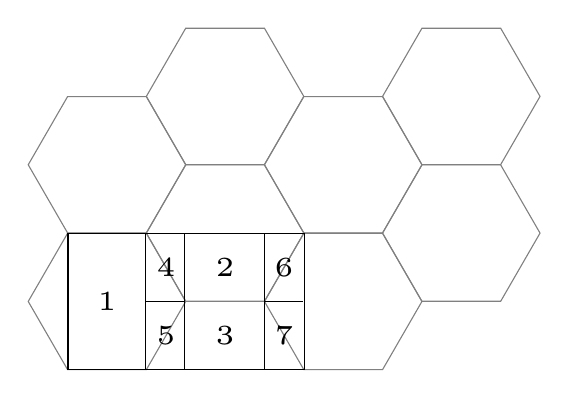
\begin{tikzpicture}[x=7.5mm,y=4.34mm, scale=2, every node/.style={scale=2}]


 \tikzset{
    box/.style={
      regular polygon,
      regular polygon sides=6,
      minimum size=10mm,
      inner sep=0mm,
      outer sep=0mm,
      rotate=0,
    draw
    }
  }
  

\foreach \i in {0,...,1} 
    \foreach \j in {0,...,1} {
            \node[box, color=gray] at (2*\i,2*\j) {};
            \node[box, color=gray] at (2*\i+1,2*\j+1) {};
        }



\draw  (-0.33,-1) rectangle (1.67,1);

\draw (0.33,-1) -- (0.33,1);
\draw (0.66,-1) -- (0.66,1);
\draw (1.33,-1) -- (1.33,1);

\draw (0.66,0) -- (0.33,0);
\draw (1.33,0) -- (1.66,0);

\node at (0,0) {\tiny{1}};
\node at (1,0.5) {\tiny{2}};
\node at (1,-0.5) {\tiny{3}};
\node at (0.5,0.5) {\tiny{4}};
\node at (0.5,-0.5) {\tiny{5}};
\node at (1.5,0.5) {\tiny{6}};
\node at (1.5,-0.5) {\tiny{7}};

\end{tikzpicture}
\caption{Link from hexagon coordinates to positions in a matrix}
\label{tkz:hex2matrix}
\end{figure}


\end{document}